\section{Matrix Multiplication Implementation}

% Should this even be here?
Matrix multiplication can be done sequentially in time complexity $O(l * m * n)$. For square matrices this can be expressed as $O(n^3)$ for $n^2$ data. For each element $n$ many independent operations have to be performed. Because these operations are independent, they can be computed in parallel. This can, potentially, have a large positive impact on performance. % Er det rigtigt at det er n independent operations? Det er vel nærmere at det er n operationer pr. element som kan køres uafhængigt af de andre elementer i matricen.

\subsection{Multiplication: CPU Implementation}
The implementation follows a standard sequential procedure with a triple nested for loop. For each element in the output matrix, a row from input matrix A is paired with a column from input matrix B as illustrated in Figure \ref{fig:multiplication_illustration}. The sum of all products of each pair of elements from A[i] and B[j] will be the result C[i][j]. % B[j] ligner at man indexerer i jth row på B. Det bør vi skrive på en anden måde, så man forstår at det er en column.
In this implementation, a single CPU thread will compute the entire result matrix.

\begin{lstlisting}[language=C, caption={Matrix Multiplication on the CPU}, label={lst:matrix_multiplication_cpu}]
bool matrix_multiplication(matrix_t *matrix_a, matrix_t *matrix_b, matrix_t *matrix_c) {
    // input validation and variable declarations { ... }
    for (int i = 0; i < result_rows; i++)
        for (int j = 0; j < result_columns; j++) {
            sum_of_products = 0.0f;
            for (int k = 0; k < common_dimension_length; k++) // consider renaming to m
                sum_of_products +=
                    matrix_a->values[INDEX(i, k, matrix_a_columns)] *
                    matrix_b->values[INDEX(k, j, matrix_b_columns)];
            matrix_c->values[INDEX(i, j, result_columns)] = sum_of_products;
        }
    return true;
}
\end{lstlisting}


\subsection{Multiplication: GPU Implementation Single Core}
The same procedure is implemented on the GPU, to compare the single core version from the CPU with the GPU.

\begin{lstlisting}[language=C, caption={Matrix Multiplication on the gpu}, label={lst:matrix_multiplication_gpu}]
__global__ void cuda_matrix_multiplication_single_core_kernel(
    device_matrix_t matrix1, device_matrix_t matrix2, device_matrix_t result,
    int l, int n, int m) {
    float sum_of_products;

    for (int i = 0; i < l; i++)
        for (int j = 0; j < n; j++) {
            sum_of_products = 0.0f;
            for (int k = 0; k < m; k++)
                sum_of_products +=
                    matrix1[INDEX(i, k, m)] * matrix2[INDEX(k, j, n)];
            result[INDEX(i, j, n)] = sum_of_products;
        }
}
\end{lstlisting}

The following three sections will explore various approaches to improve runtime performance by utilizing the GPU architecture in different ways. % Vi bør også snakke om block_size og grid_size er 1, og at dette betyder at vi ikke kan regne på større matricer end 1024

\subsection{Multiplication: GPU Implementation Multi Core}

% Bør vi måske kalde den Multi Block i stedet for Multi Core? Sv: Den er jo multi core

In this version, we aim to utilize the block architecture of the GPU. We initialize our grid to be one dimensional with $l$ many blocks, where $l$ is the number of rows in the result matrix. Each block has a single thread.

One thread (and block) is then responsible for computing one column of the result matrix. This essentially \textit{unwraps} the outermost for-loop (using i as the counter), which was previously iterating over all rows. Therefore this implementation is dubbed "unwrapping i". One is then left with a single nested for-loop, as can be seen in listing \ref{lst:matrix_multiplication_gpu_multi_core}.

\begin{lstlisting}[language=C, caption={Multi Core Matrix Multiplication}, label={lst:matrix_multiplication_gpu_multi_core}]
__global__ void cuda_matrix_multiplication_multicore_unwrapping_i_kernel(
    device_matrix_t matrix_a, device_matrix_t matrix_b,
    device_matrix_t matrix_c, int l, int n, int m) {

    int i = blockIdx.x;
    float sum_of_products;
    for (int j = 0; j < n; j++) {
        sum_of_products = 0.0f;
        for (int k = 0; k < m; k++)
            sum_of_products +=
                matrix_a[INDEX(i, k, m)] * matrix_b[INDEX(k, j, n)];
        matrix_c[INDEX(i, j, n)] = sum_of_products;
    }
}
\end{lstlisting}

\subsection{Multiplication: GPU Implementation Multi Core 2}

% Bør vi måske kalde den Multi Block Multi Thread i stedet for Multi Core 2?

Taking this one step further, we will now utilize that each block can have many threads. Specifically, we will spawn $n$ many threads in each block, where $n$ is the number of columns in the result matrix. 

This way, each thread will be responsible for calculating on one single element of the result matrix. The block determines which row, and the thread determines which column. This leaves us with a kernel that has only a single for-loop as can be seen in listing \ref{lst:matrix_multiplication_gpu_multi_core_multi_thread}. 

\begin{lstlisting}[language=C, caption={Multi Core Multi Thread Matrix Multiplication}, label={lst:matrix_multiplication_gpu_multi_core_multi_thread}]
__global__ void cuda_matrix_multiplication_multicore_unwrapping_i_and_j_kernel(
    device_matrix_t matrix_a, device_matrix_t matrix_b,
    device_matrix_t matrix_c, int l, int n, int m) {
    int i = blockIdx.x;
    int j = threadIdx.x;
    float sum_of_products = 0.0f;

    for (int k = 0; k < m; k++)
        sum_of_products += matrix_a[INDEX(i, k, m)] * matrix_b[INDEX(k, j, n)];

    matrix_c[INDEX(i, j, n)] = sum_of_products;
}
\end{lstlisting}

A limitation to this approach is that the maximum block size is 1024, meaning if we try to compute a matrix multiplication where $n$ is greater than 1024, it simply will not work. Our next section will rectify this limitation.

\subsection{Multiplication: GPU Implementation Shared Memory}

% Reference Variable Memory Space Specifiers: https://docs.nvidia.com/cuda/cuda-c-programming-guide/index.html#variable-memory-space-specifiers

In this implementation, we aim to utilize the memory architecture of the GPU. As seen back in figure \ref{fig:cpu_vs_gpu}, all blocks have access to global DRAM and an L2 cache. However, each block also has access to its own much faster local L1 cache, although it is much limited in size when compared. 

The key observation is that each element in matrix A will be accessed $n$ many times, and each element in matrix B will be accessed $l$ many times. For each computed element in matrix C, this means $2m$ many reads. And to compute a full matrix, this means $2m * n * l$ many reads. For each time we want to access an element we have to query the global DRAM. This will be the bottle neck of our algorithm. 

For this implementation, each thread will still only be responsible for calculating a single element in the result matrix. However, our blocks will be defined by threads, that access much of the same memory. These threads will help each other retrieve the commonly accessed values from matrix A and B. By doing this, the L1 cache is filled in parallel with the commonly accessed memory, so that all threads can quickly access it and compute their values. 


\color{red} Insert sentences on how much space the L1 cache has, how many floats that is and the calculation that determines BLOCK\_SIZE \color{black}

Previously we have only accessed our blocks and threads by their x-coordinate. For this implementation, it helps to abstract the memory access to be 2-dimensional. That means we will start to access our specific blocks and threads with both x- and y-coordinates. 

Now that we have tiled our blocks to cover the grid, we will concentrate on a single arbitrary block. This block has $GRID\_SIZE$ * $GRID\_SIZE$ many threads. Each block will have 2 corresponding sub matrices, also of size $GRID\_SIZE$ * $GRID\_SIZE$. These will be declared as \_\_shared\_\_ float 2D-arrays. This keyword in CUDA-C tells the compiler to put this memory on the shared L1 cache, such that all threads within the block has access to it. 
The next step of the algorithm is to loop through $m / GRID\_SIZE$ many squares of matrix A and matrix B. For each iteration, each thread will write one value from A and B to these shared matrices. With these in place, each thread can now sum up GRID\_SIZE many products. Doing this in $m / GRID\_SIZE$ many iterations will allow each thread to calculate the full matrix product and store the result in matrix C. 

\begin{figure}[ht]
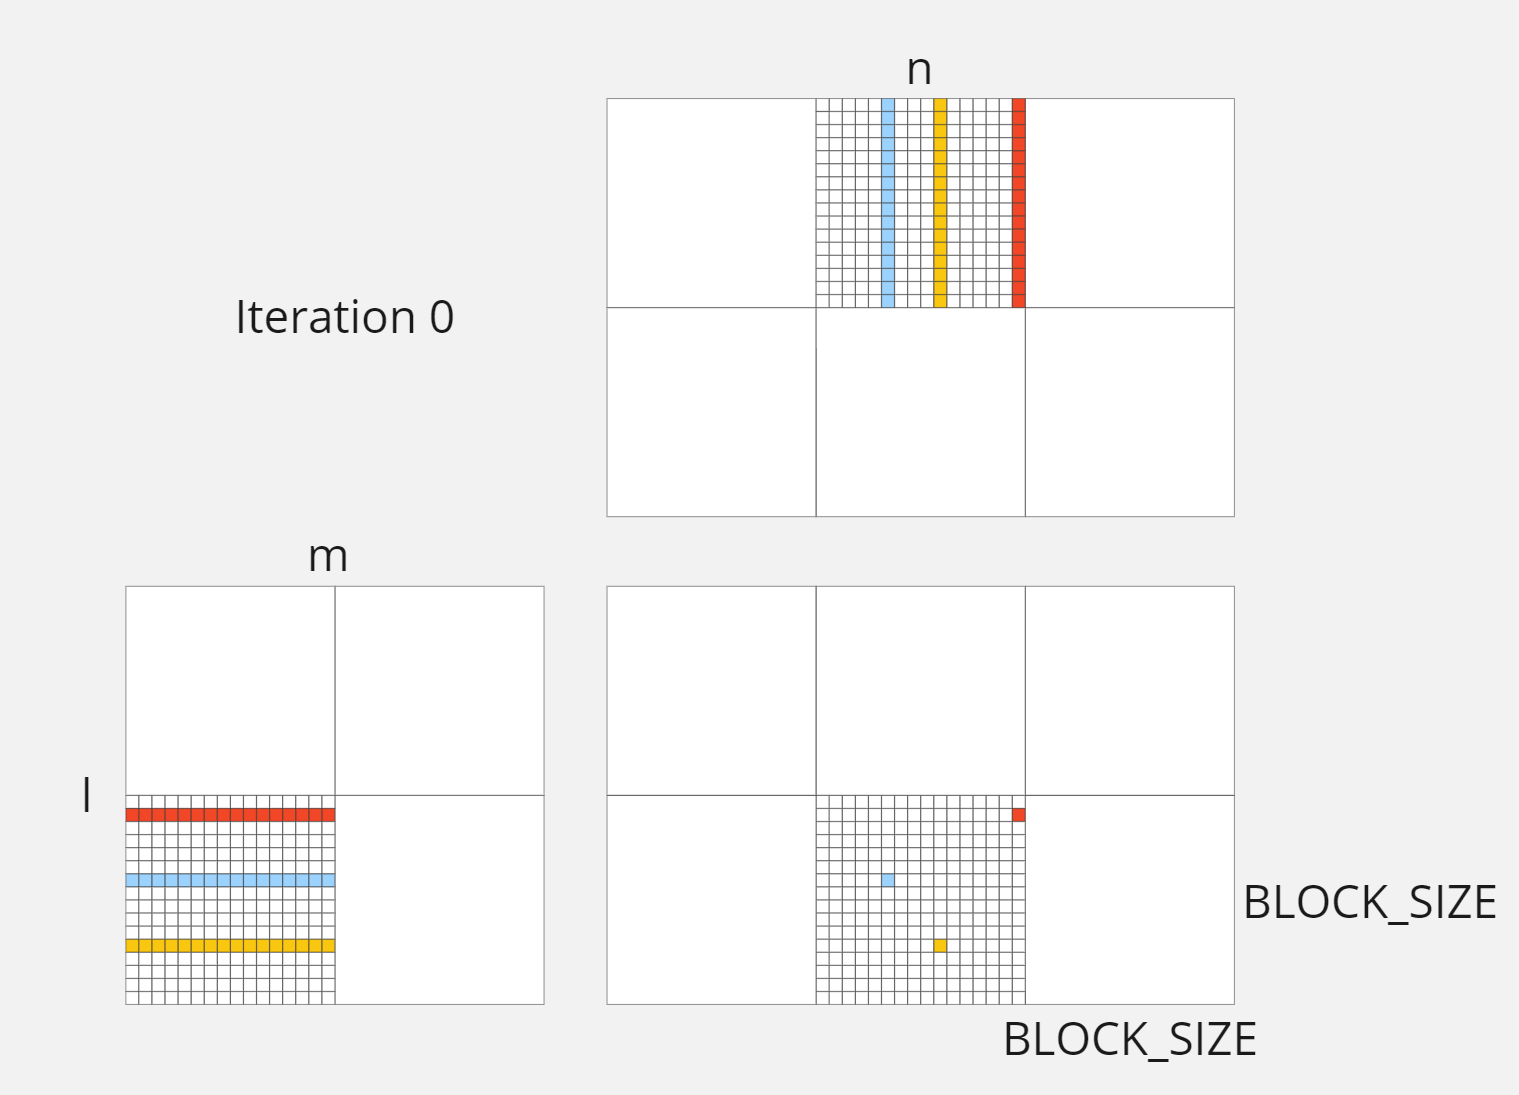
\includegraphics[width=\textwidth]{Documents/Report/Figures/SharedMemory1.png}
\label{fig:threads and blocks.}
\end{figure}

\begin{figure}[ht]
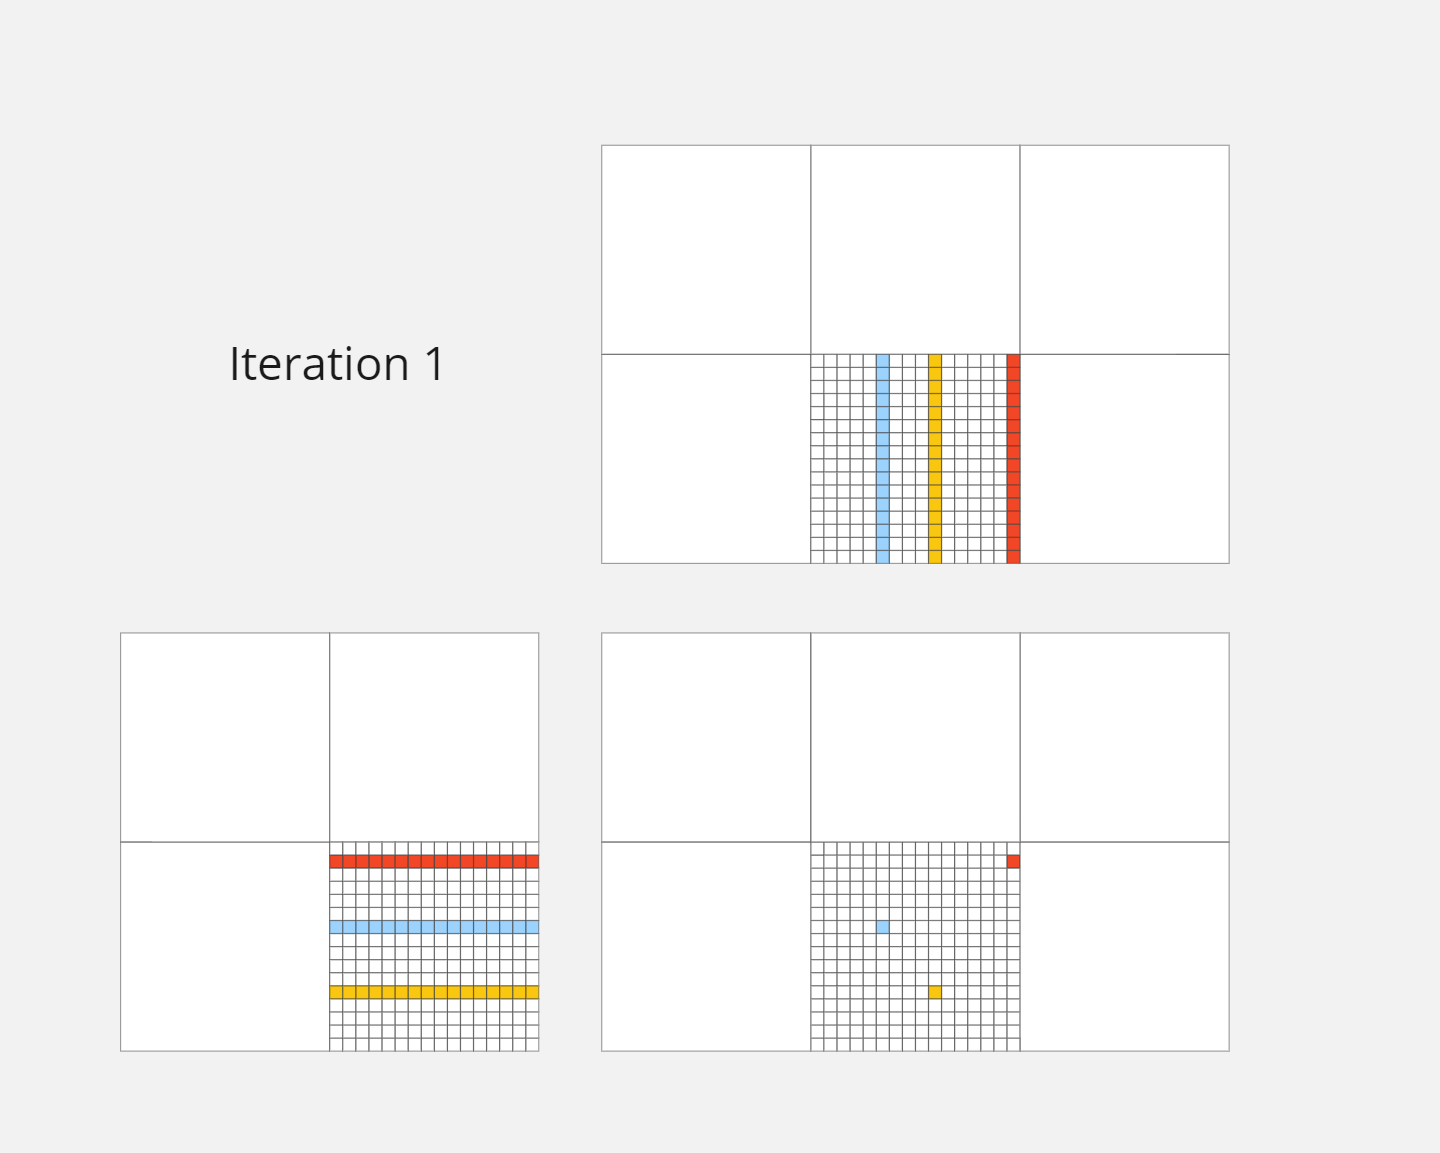
\includegraphics[width=\textwidth]{Documents/Report/Figures/SharedMemory2.png}
\label{fig:threads and blocks 2.}
\end{figure}

To avoid race conditions, we use the CUDA specific method $\_\_syncthreads$ to synchronize the threads. In each iteration it is called first to make sure all values of matrix A and B are retrieved before using them for calculations. It is called one more time to ensure all threads are done using the values before they are overwritten again for the next iteration. See the implementation below. 

\begin{lstlisting}[language=C, caption={Shared Memory Matrix Multiplication}, label={lst:matrix_multiplication_gpu_shared_memory}]
__global__ void cuda_matrix_multiplication_multicore_unwrapping_i_and_j_kernel(
    device_matrix_t matrix_a, device_matrix_t matrix_b,
    device_matrix_t matrix_c, int l, int n, int m) __global__ void cuda_matrix_multiplication_multi_core_shared_memory_kernel(
    device_matrix_t matrix_a, device_matrix_t matrix_b,
    device_matrix_t matrix_c, int l, int n, int m) {
    
    int block_row = blockIdx.y;
    int block_column = blockIdx.x;
    int row = threadIdx.y;
    int column = threadIdx.x;
    float c_value = .0f;

    int subs_in_m = (m + BLOCK_SIZE - 1) / BLOCK_SIZE;
    for (int k = 0; k < subs_in_m; k++) {
        device_matrix_t a_sub = get_sub_matrix(matrix_a, block_row, k, m);
        __shared__ float shared_a_sub[BLOCK_SIZE][BLOCK_SIZE];
        shared_a_sub[row][column] = a_sub[INDEX(row, column, m)];

        device_matrix_t b_sub = get_sub_matrix(matrix_b, k, block_column, n);
        __shared__ float shared_b_sub[BLOCK_SIZE][BLOCK_SIZE];
        shared_b_sub[row][column] = b_sub[INDEX(row, column, n)];
        __syncthreads();

        for (int i = 0; i < BLOCK_SIZE; i++) 
            c_value += shared_a_sub[row][i] * shared_b_sub[i][column];
        __syncthreads();
    }

    if (row + BLOCK_SIZE * block_row < l && column + BLOCK_SIZE * block_column  < n) {
        device_matrix_t c_sub = get_sub_matrix(matrix_c, block_row, block_column, n);
        c_sub[INDEX(row, column, n)] = c_value;
    } 
}
\end{lstlisting}

VIGTIGT: Vi skal huske at nævne at implementationen er strækt inspireret af NVIDIAs dokumentation.

% Define shared A sub and B sub
% Define how they move across matrix C in m / block_size iterations, moving shared subs for every iteration
% Explain how in each iteration, one thread retrives one value from global memory/DRAM L2 and puts it in local memory/L1
% When shared sub a and b are filled out, (sync threads), each thread's c_value is added to
% When shared a and b have moved all the way through m, c_value is calculated and can be stored in global memory.

